\documentclass[12pt]{article}
\usepackage[utf8]{inputenc}
\usepackage[russian]{babel}
\usepackage{amsmath}
\usepackage{amssymb}
\usepackage{amsthm}
\usepackage{indentfirst}
\usepackage{graphicx}
\usepackage{multicol}
\usepackage{dsfont}
\usepackage{color}
\usepackage[left=2.5cm,right=2.5cm,top=2cm,bottom=2cm,bindingoffset=0cm,columnsep=1cm]{geometry}
\usepackage{systeme}
\usepackage{epsfig}
\usepackage{mathrsfs}
\usepackage{bbm}

\usepackage{fancybox,fancyhdr}
\pagestyle{fancy}



\fancyhead[R]{Михаил Минин}
\fancyhead[L]{09.12.2024}
\fancyhead[C]{Тестовое / Data analyst}

\theoremstyle{indented}                                                                              
\newtheorem{theorem}{Теорема}
\newtheorem{lemma}{Лемма}
\theoremstyle{definition} 
\newtheorem{dfn}{Определение}
\newtheorem{ex}{Пример(ы)}
\theoremstyle{remark} 
\newtheorem{remark}{Примечание}
\newtheorem{prop}{Свойствo}
\newtheorem{cons}{Следствие}


\begin{document}

Все файлы проекта: https://github.com/Mihey-38/test\_task\_for\_DA

\section{Уменьшение времени подтверждения транзакций BTC}

Проблема: Партнёр отказывается процессить обмены из BTC, так как транзакции занимают более 20 минут из-за ожидания подтверждений и риска реорганизации цепи.

\subsection*{Предложенные решения}
Для минимизации времени подтверждения транзакций и снижения рисков предлагаются следующие подходы:

\begin{enumerate}
    \item \textbf{Уменьшение количества необходимых подтверждений:}
    \begin{itemize}
        \item Для транзакций с небольшими суммами снизить количество требуемых подтверждений до 1-2.
        \item Для крупных сумм использовать более консервативные настройки (например, 3-6 подтверждений).
    \end{itemize}
    Какие суммы можно считать <<небольшими>>? \\
    Если потери из-за реорганизации для суммы $x$ больше стоимости потенциального отказа партнёра, то такую сумму можно считать <<небольшой>>.

    \item \textbf{Использование решений второго уровня (Lightning Network):}
    \begin{itemize}
        \item Lightning Network позволяет проводить мгновенные транзакции без необходимости ожидания подтверждений в блокчейне.
        \item Для крупных или редко используемых сумм можно предусмотреть автоматический переход на основную цепочку.
    \end{itemize}

    \item \textbf{Страхование рисков реорганизации цепи:}
    \begin{itemize}
        \item Внедрить механизм страхования, покрывающий возможные убытки из-за реорганизации цепи.
        \item Использовать мониторинг сети для оперативного выявления риска реорганизации.
    \end{itemize}
    На практики реорганизации в сети Bitcoin очень редки и маловероятны.
\end{enumerate}

\subsection*{Отслеживаемые метрики}
Для контроля эффективности решений и управления рисками предлагается отслеживать следующие показатели:
\begin{itemize}
    \item Среднее время подтверждения транзакции (в минутах).
    \item Частота реорганизаций цепи (количество реорганизаций за определённый период).
    \item Объем средств, обработанных с уменьшенным количеством подтверждений.
    \item Процент транзакций, отклонённых из-за превышения времени подтверждения.
    \item Общая сумма транзакций, обработанных с уменьшенным количеством подтверждений.
\end{itemize}

\newpage

\section{Увеличение оборотов сервиса}

Задача: определить, каких активов на сервисе не хватает, и выделить активы, на которые стоит сфокусироваться с точки зрения маркетинга и бизнес-девелопмента. Цель — увеличить обороты сервиса.

\subsection*{Методика анализа}
\subsection*{1. Сбор данных}
\begin{itemize}
    \item Из внутренней базы сервиса: данные об оборотах текущих активов.
    \item Из внешних источников, например CoinMarketCap:
    \begin{itemize}
        \item Рыночная капитализация активов,
        \item Объем торгов за сутки,
        \item Количество бирж, поддерживающих актив,
        \item Региональные предпочтения.
    \end{itemize}
\end{itemize}

\subsubsection*{2. Сравнение текущего ассортимента сервиса с внешними данными}
\begin{itemize}
    \item Составить список активов, отсутствующих на сервисе.
    \item Определить популярность отсутствующих активов по следующим критериям:
    \begin{itemize}
        \item Высокий объем торгов за сутки.
        \item Растущий тренд рыночной капитализации.
        \item Популярность в регионах, где находится основная аудитория сервиса.
    \end{itemize}
\end{itemize}

\subsubsection*{3. Приоритизация активов}
Для определения приоритетов добавления активов следует:
\begin{itemize}
    \item Рассчитать рейтинг по формуле:
    \[
    R = \alpha \cdot V_{24h} + \beta \cdot MC + \gamma \cdot T,
    \]
    где:
    \begin{itemize}
        \item $R$ — общий рейтинг актива.
        \item $V_{24h}$ — объем торгов за сутки.
        \item $MC$ — рыночная капитализация.
        \item $T$ — тренд популярности (например, процентный рост за месяц).
        \item $\alpha, \beta, \gamma$ — веса, определяющие важность каждого фактора.
    \end{itemize}
    \item Составить таблицу с результатами и выделить топ-активы для добавления.
\end{itemize}

\subsection*{Метрики для отслеживания эффективности}
Для контроля успешности предложенной методики предлагается отслеживать следующие метрики:
\begin{itemize}
    \item Объем торгов новых активов, добавленных на платформу.
    \item Доля активов с растущим трендом (положительное изменение оборота).
    \item Увеличение общего оборота платформы (в процентном выражении).
\end{itemize}

\newpage

\section{Анализ SQL-запроса}

\subsection{Из каких таблиц какие берутся данные?}

Запрос извлекает данные из следующих таблиц:
\begin{itemize}
    \item \textbf{iof (in\_out\_flow):}
    \begin{itemize}
        \item \texttt{contract\_id} — уникальный идентификатор контракта.
        \item \texttt{flow\_in} — объём входящих средств.
        \item \texttt{flow\_out} — объём исходящих средств.
        \item \texttt{timestamp} — временная метка транзакции.
    \end{itemize}
    \item \textbf{t (totals):}
    \begin{itemize}
        \item \texttt{contract\_id} — уникальный идентификатор контракта.
        \item \texttt{partner\_id} — идентификатор партнёра.
        \item \texttt{total\_profit} — прибыль, связанная с данным контрактом.
    \end{itemize}
\end{itemize}


\subsection{Как изменить запрос для партнёра с \texttt{partner\_id = 137}?}

Чтобы выбрать данные только по партнёру с идентификатором \texttt{partner\_id = 137}, нужно заменить условие \texttt{WHERE}:

\begin{verbatim}
WHERE t.partner_id IN (1, 2, 3)
\end{verbatim}

на:

\begin{verbatim}
WHERE t.partner_id = 137
\end{verbatim}

\newpage

\section{Скрипт для анализа данных с CoinMarketCap\\ и SimpleSwap}

\subsection*{Описание работы кода}
Код выполняет последовательный анализ данных из двух источников — CoinMarketCap и SimpleSwap для выявления криптовалют, которые отсутствуют на платформе SimpleSwap. Далее производится сортировка по суточному объему торгов, чтобы определить приоритетные активы для добавления.

\subsection*{Пошаговое описание}

\subsection{Получение данных с CoinMarketCap}
\begin{itemize}
    \item Отправляем HTTP-запрос к API CoinMarketCap для получения данных о первых 1500 криптовалютах, отсортированных по рыночной капитализации.
    \item Из API возвращается информация о каждой криптовалюте, включая её название, символ, объемы торгов за сутки, рыночную капитализацию и другие метрики.
\end{itemize}

\subsection{Преобразование данных в табличный формат}
\begin{itemize}
    \item Полученные данные преобразуем в pandas-DataFrame.
\end{itemize}

\subsection{Проверка структуры данных}
\begin{itemize}
    \item Выводим список всех доступных столбцов в таблице, чтобы понять, какие данные предоставляет API.
    \item Эта проверка важна для дальнейшего извлечения нужных метрик, таких как объем торгов за сутки (\texttt{volume24h}).
\end{itemize}

\subsection{Извлечение объема торгов за сутки}
\begin{itemize}
    \item Код проверяет наличие столбца, содержащего торговые метрики (например, \texttt{quotes}).
    \item Если столбец существует, из него извлекается значение \texttt{volume24h}, отражающее суточный объем торгов каждой криптовалюты.
\end{itemize}

\subsection{Фильтрация данных CoinMarketCap}
\begin{itemize}
    \item Из всей таблицы оставляем только три ключевых столбца:
    \begin{itemize}
        \item Символ криптовалюты (\texttt{symbol}).
        \item Название криптовалюты (\texttt{name}).
        \item Суточный объем торгов (\texttt{volume24h}).
    \end{itemize}
\end{itemize}

\subsection{Получение данных с SimpleSwap}
\begin{itemize}
    \item Отправляем запрос к API SimpleSwap для получения списка всех криптовалют, поддерживаемых на платформе.
    \item Полученные данные преобразуем в множество (\textit{set}) символов криптовалют, доступных на SimpleSwap.
\end{itemize}

\subsection{Поиск криптовалют, отсутствующих на SimpleSwap}
\begin{itemize}
    \item Таблицу CoinMarketCap сравниваем с данными SimpleSwap.
    \item Удаляем записи о криптовалютах, символы которых уже есть в SimpleSwap.
    \item Таким образом, формируется список криптовалют, которых нет на SimpleSwap.
\end{itemize}

\subsection{Сортировка по суточному объему торгов}
\begin{itemize}
    \item Сортируем криптовалюты, отсутствующие на SimpleSwap по убыванию объема торгов за сутки (\texttt{volume24h}).
\end{itemize}

\subsection{Вывод результатов}
\begin{itemize}
    \item Выводим итоговую таблицу с отсутствующими криптовалютами, отсортированными по суточному объему торгов.
\end{itemize}

\section*{Приложение 1: Скрипт}
\begin{verbatim}
import requests
import pandas as pd

cmc_url = "https://api.coinmarketcap.com/data-api/v3/cryptocurrency/listing?start=1&limit=1500&sortBy=market_cap&sortType=desc&convert=USD,BTC,ETH&cryptoType=all&tagType=all&audited=false&aux=ath,atl,high24h,low24h,num_market_pairs,cmc_rank,date_added,max_supply,circulating_supply,total_supply,volume_7d,volume_30d,self_reported_circulating_supply,self_reported_market_cap"
cmc_data = requests.get(cmc_url).json()["data"]["cryptoCurrencyList"]

cmc_df = pd.DataFrame(cmc_data)

print("Доступные столбцы:", cmc_df.columns)


# В консоли вернулось:

# Доступные столбцы: Index(['id', 'name', 'symbol', 'slug', 'cmcRank', 'marketPairCount',
#        'circulatingSupply', 'selfReportedCirculatingSupply', 'totalSupply',
#        'maxSupply', 'ath', 'atl', 'high24h', 'low24h', 'isActive',
#        'lastUpdated', 'dateAdded', 'quotes', 'isAudited', 'auditInfoList',
#        'badges'],
#       dtype='object')

# Скорее всего, объем торгов за сутки будет в "quotes" 


print(cmc_df['quotes'][0])
if "quotes" in cmc_df.columns:
    cmc_df["volume24h"] = cmc_df["quotes"].apply(lambda x: x[0]["volume24h"] if x else None)


cmc_df = cmc_df[["symbol", "name", "volume24h"]]

ss_url = "https://simpleswap.io/api/v3/currencies?fixed=false&includeDisabled=false"
ss_data = requests.get(ss_url).json()

ss_symbols = {coin["symbol"] for coin in ss_data}
print('Всего монет в simpleswap:', len(ss_symbols))

missing_coins = cmc_df[~cmc_df["symbol"].isin(ss_symbols)]

sorted_missing_coins = missing_coins.sort_values(by="volume24h", ascending=False)

print(sorted_missing_coins)
\end{verbatim}

\section*{Приложение 2: результат исполнения}
\begin{center}
    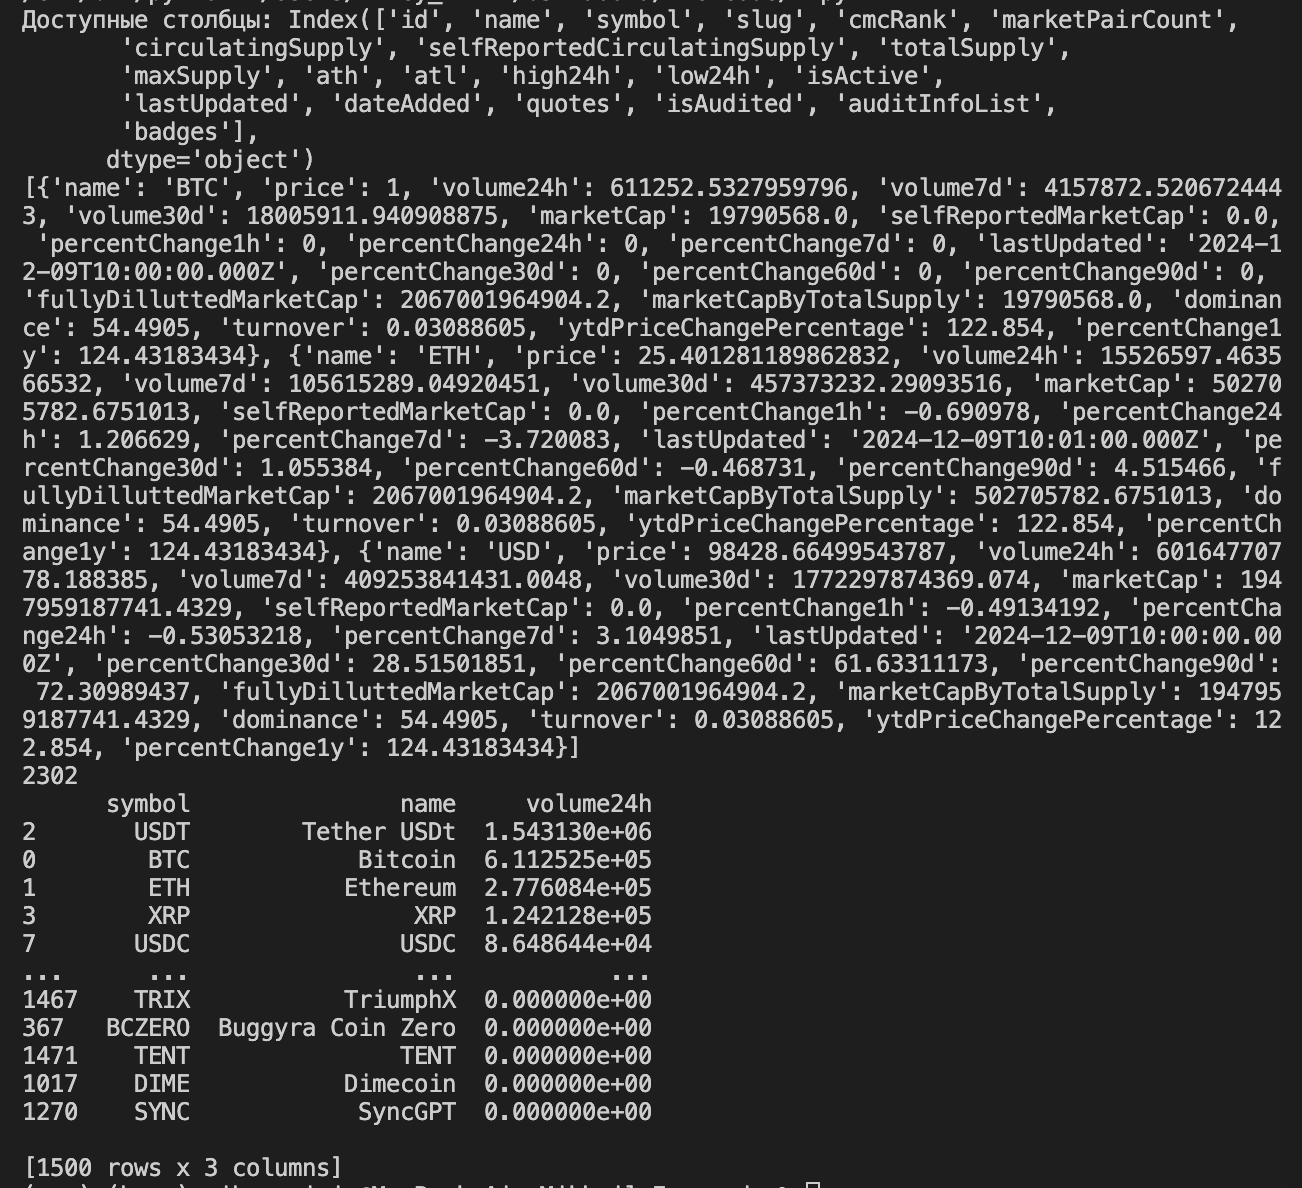
\includegraphics[width = 1.0\textwidth]{output.png}
\end{center}



\end{document}